\documentclass{article}
\usepackage{amsmath}
\usepackage{amsfonts}
\usepackage{parskip}
\usepackage{svg}
\usepackage[utf8]{inputenc}
\usepackage{helvet}
\renewcommand{\familydefault}{\sfdefault}
\usepackage{geometry}
\usepackage[document]{ragged2e}
\geometry{letterpaper, portrait, top=1in, bottom=1in, left=1.5in, right=1.5in}

\title{Math 301}

\begin{document}

\section{Set Notation}
\begin{align*}
    \mathbb{N} &= natural\ numbers = \{0, 1, 2 \cdots\} \\
    \mathbb{Z} &= integers = \{ \cdots -2, -1, 0, 1, 2 \cdots \}\\
    \mathbb{Q} &= rational\ numbers\ (can\ be\ expressed\ with\ fractions\ of\ two\ integers) \\
    \mathbb{R} &= real\ numbers\ (rational\ numbers\ and\ irrational\ numbers)
\end{align*}

A is an element of B
\begin{gather*}
    A \in B
\end{gather*}

A is a subset of b
\begin{gather*}
    A \subseteq B
\end{gather*}

The cardinality of A
\begin{gather*}
    |A|
\end{gather*}

Complement of A
\begin{gather*}
    A^C \\
    \overline{A}
\end{gather*}

The intersection of A and B
\begin{gather*}
    A \cap B
\end{gather*}

The union of A and B
\begin{gather*}
    A \cup B
\end{gather*}

The symmetric difference of A and B
\begin{gather*}
    A \oplus B = (A \cup B) - (A \cap B)
\end{gather*}

\section{Cartesian Products}

The Cartesian product of A and B
\begin{gather*}
    A \times B = {(a, b) | a \in A, b \in B}
\end{gather*}

\begin{gather*}
    |A \times B| = |A| \times |B|
\end{gather*}

The power set of A is the set of all subsets of A.
\begin{gather*}
    \mathcal{P}(A)
\end{gather*}

\begin{gather*}
    |\mathcal{P}(A)| = 2^{|A|}
\end{gather*}

\section{The Rule of Products}
Given the number of possibilities for two independent events denoted $|A|$ and $|B|$, the number of possible combinations of both events is $|A| \times |B|$. You can also say "the number of ways to do $A$ \textbf{AND} $B$ is $|A| \times |B|$."

\section{The Law of Addition}

The basic law of addition
\begin{gather*}
    |A| = |A_1| + |A_2| + \cdots + |A_n| = \sum_{k=1}^{n} |A_k|
\end{gather*}

Given the number of possibilities for two mutually exclusive events denoted $|A|$ and $|B|$, the sum of possible events is $|A| + |B|$. "The number of ways to do $A$ \textbf{OR} $B$ is $|A| + |B|$."

Partition of a set
\begin{gather*}
    A_1 \cup A_2 \cup A_3 \cup \cdots = A \\
    A_i \cap A_j = \emptyset\ where\ i \neq j\
\end{gather*}

Law of inclusion-exclusion for two sets

\begin{gather*}
    |A_1 \cup A_2| = |A_1| + |A_2| - |A_1 \cap A_2|
\end{gather*}

\begin{gather*}
\end{gather*}

\section{Permutation}
The total number of ordered sets of $k$ elements taken from a set of $n$ elements
\begin{gather*}
    P(n,k) = \frac{n!}{(n-k)!}
\end{gather*}

\section{Combination}
The total number of unordered sets of $k$ elements taken from a set of $n$ elements
\begin{gather*}
    \binom{n}{k} = \frac{n!}{(n-k)!k!}
\end{gather*}

Binomial theorem---Allows you to expand $(x+y)^n$.
\begin{gather*}
    (x + y)^n = \sum_{k=0}^{n} \binom{n}{k}x^{n-k}y^k
\end{gather*}

\section{Logical operator}

Logical conjunction (AND)
\begin{gather*}
    p \land q \\
    \begin{tabular}{c|c|c}
        p & q & $p \land q$ \\
        \hline
        0 & 0 & 0 \\
        0 & 1 & 0 \\
        1 & 0 & 0 \\
        1 & 1 & 1
    \end{tabular}
\end{gather*}

Logical disjunction (OR)
\begin{gather*}
    p \lor q \\
    \begin{tabular}{c|c|c}
        p & q & $p \lor q$ \\
        \hline
        0 & 0 & 0 \\
        0 & 1 & 1 \\
        1 & 0 & 1 \\
        1 & 1 & 1
    \end{tabular}
\end{gather*}

Logical negation
\begin{gather*}
    \neg p \\
    \begin{tabular}{c|c}
        p & $\neg p$ \\
        \hline
        0 & 1 \\
        1 & 0
    \end{tabular}
\end{gather*}

Conditional statement (if $p$ is true then $q$ is also true)
\begin{gather*}
    p \rightarrow q \\
    \begin{tabular}{c|c|c}
        p & q & $p \rightarrow q$ \\
        \hline
        0 & 0 & 1 \\
        0 & 1 & 1 \\
        1 & 0 & 0 \\
        1 & 1 & 1
    \end{tabular}
\end{gather*}

Converse
\begin{gather*}
    p \leftarrow q \\
    or \\
    q \rightarrow p
\end{gather*}

Contrapositive
\begin{gather*}
    \neg q \rightarrow \neg p \\
    \begin{tabular}{c|c|c}
        p & q & $\neg q \rightarrow \neg p$ \\
        \hline
        0 & 0 & 1 \\
        0 & 1 & 1 \\
        1 & 0 & 0 \\
        1 & 1 & 1
    \end{tabular}
\end{gather*}

Biconditional (XNOR)
\begin{gather*}
    p \leftrightarrow q \\
    \begin{tabular}{c|c|c}
        p & q & $p \leftrightarrow q$ \\
        \hline
        0 & 0 & 1 \\
        0 & 1 & 0 \\
        1 & 0 & 0 \\
        1 & 1 & 1
    \end{tabular}
\end{gather*}

Sheffer stroke (NAND)
\begin{gather*}
    p | q \\
    \begin{tabular}{c|c|c}
        p & q & $p | q$ \\
        \hline
        0 & 0 & 1 \\
        0 & 1 & 1 \\
        1 & 0 & 1 \\
        1 & 1 & 0
    \end{tabular}
\end{gather*}

Order of precedence of propositions
\begin{enumerate}
    \item Parentheses
    \item Negation
    \item Conjunction
    \item Disjunction
    \item Conditional statement
    \item Biconditional
\end{enumerate}

\section{Equivalence and implication}

Tautology: An expression that is true in all cases

Contradiction: An expression that is false for all cases

Equivalence ($r \leftrightarrow s$ is a tautology)
\begin{gather*}
    r \Leftrightarrow s
\end{gather*}

Implication (r implies s)
\begin{gather*}
    r \Rightarrow s
\end{gather*}

\section{Laws of logic}

Duality principle: Each law of logic can be used to derive a second law by switching the symbols $\land$ with $\lor$, $1$ with $0$ and visa versa.

Commutative laws
\begin{gather*}
    p \lor q \Leftrightarrow q \lor p \\
    p \land q \Leftrightarrow q \land p
\end{gather*}

Associative laws
\begin{gather*}
    (p \lor q) \lor r \Leftrightarrow p \lor (q \lor r) \\
    (p \land q) \land r \Leftrightarrow p \land (q \land r)
\end{gather*}

Distributive laws
\begin{gather*}
    p \land (q \lor r) \Leftrightarrow (p \land q) \lor (p \land r) \\
    p \lor (q \land r) \Leftrightarrow (p \lor q) \land (p \lor r) \\
\end{gather*}

Identity laws
\begin{gather*}
    p \lor 0 \Leftrightarrow p \\
    p \land 1 \Leftrightarrow p
\end{gather*}

Negation laws
\begin{gather*}
    p \land \neg p \Leftrightarrow 0 \\
    p \lor \neg p \Leftrightarrow 1
\end{gather*}

Idempotent laws
\begin{gather*}
    p \lor p \Leftrightarrow p \\
    p \land p \Leftrightarrow p
\end{gather*}

Null laws
\begin{gather*}
    p \land 0 \Leftrightarrow 0 \\
    p \lor 1 \Leftrightarrow 1
\end{gather*}

Absorption laws
\begin{gather*}
    p \land (p \lor q) \Leftrightarrow p \\
    p \lor (p \land q) \Leftrightarrow p
\end{gather*}

DeMorgan's laws
\begin{gather*}
    \neg (p \lor q) \Leftrightarrow (\neg p) \land (\neg q) \\
    \neg (p \land q) \Leftrightarrow (\neg p) \lor (\neg q)
\end{gather*}

Involution law
\begin{gather*}
    \neg (\neg p) \Leftrightarrow p
\end{gather*}

Detachment
\begin{gather*}
    (p \rightarrow q) \land p \Rightarrow q
\end{gather*}

Indirect reasoning
\begin{gather*}
    (p \rightarrow q) \land \neg q \Rightarrow \neg p
\end{gather*}

Disjunctive addition
\begin{gather*}
    p \Rightarrow (p \lor q)
\end{gather*}

Conjunctive simplification
\begin{gather*}
    (p \land q) \Rightarrow p \\
    (p \land q) \Rightarrow q
\end{gather*}

Disjunctive simplification
\begin{gather*}
    (p \lor q) \land \neg p \Rightarrow q \\
    (p \lor q) \land \neg q \Rightarrow p
\end{gather*}

Chain rule
\begin{gather*}
    (p \rightarrow q) \land (q \rightarrow r) \Rightarrow (p \rightarrow r)
\end{gather*}

Conditional equivalence
\begin{gather*}
    p \rightarrow q \Leftrightarrow \neg p \lor q
\end{gather*}

Biconditional equivalences
\begin{gather*}
    (p \leftrightarrow q) \Leftrightarrow (p \rightarrow q) \land (q \rightarrow p) \Leftrightarrow (p \land q) \lor (\neg p \land \neg q)
\end{gather*}

Contrapositive
\begin{gather*}
    (p \rightarrow q) \Leftrightarrow (\neg q \rightarrow \neg p)
\end{gather*}

\section{Propositions over a Universe}

If $p$ is a proposition over $U$, the truth set of $p$ is $T_p = \{a \in U | p(a)\ is\ true\}$.

\section{Mathematical induction}

Mathematical induction is a way to prove a proposition over natural numbers.

\begin{enumerate}
    \item Prove the basis of the statement, $P(n)$ where $n = 0$.
    \item Assume the statement is true for $n - 1$. Prove $P(n-1) \Rightarrow P(n)$.
\end{enumerate}

Stronk induction

\begin{enumerate}
    \item Prove the bases of the statement, $P(m)$, for an arbitrary $m > 0$.
    \item Assume the statement is true for $k$ where $m \leq k < n$. Prove $P(k) \Rightarrow n$.
\end{enumerate}

\section{Quantifiers}

The existential quantifier states that there exists an $n$ such that $p(n)$ is true.
\begin{gather*}
    (\exists n)(p(n))
\end{gather*}

The universal quantifier states that for all $n$ in $U$, $p(n)$ is true.
\begin{gather*}
    (\forall n)(p(n))
\end{gather*}

Negation of quantified propositions
\begin{gather*}
    \neg ((\forall n)(p(n))) \Leftrightarrow (\exists n)(\neg p(n)) \\
    \neg ((\exists n)(p(n))) \Leftrightarrow (\forall n)(\neg p(n))
\end{gather*}

Multiple quantifiers of the same type can be arranged in any order, but mixed quantifiers cannot be exchanged.

\section{Proofs for sets}

You can prove set propositions using Venn diagrams, truth tables (true indicating that $x \in A$ or with definitions.

To prove that $A \subseteq B$, show that $x \in A$ and $x \in B$. \\
To prove that $A = B$, show that $A \subseteq B$ and $B \subseteq A$.

\section{Laws of set theory}

Commutative laws
\begin{gather*}
    A \cup B = B \cup A \\
    A \cap B = B \cap A
\end{gather*}

Associative laws
\begin{gather*}
    A \cup (B \cup C) = (A \cup B) \cup C \\
    A \cap (B \cap C) = (A \cap B) \cap C
\end{gather*}

Distributive laws
\begin{gather*}
    A \cap (B \cup C) = (A \cap B) \cup (A \cap C) \\
    A \cup (B \cap C) = (A \cup B) \cap (A \cup C)
\end{gather*}

Identity laws
\begin{gather*}
    A \cup \emptyset = A \\
    A \cap U = A
\end{gather*}

Complement laws
\begin{gather*}
    A \cup \overline{A} = U \\
    A \cap \overline{A} = \emptyset
\end{gather*}

Idempotent laws
\begin{gather*}
    A \cup A = A \\
    A \cap A = A
\end{gather*}

Null laws
\begin{gather*}
    A \cup U = U \\
    A \cap \emptyset = \emptyset
\end{gather*}

Absorption laws
\begin{gather*}
    A \cup (A \cap B) = A \\
    A \cap (A \cup B) = A
\end{gather*}

DeMorgan's laws
\begin{gather*}
    \overline{A \cup B} = \overline{A} \cap \overline{B} \\
    \overline{A \cap B} = \overline{A} \cup \overline{B}
\end{gather*}

Involution law
\begin{gather*}
    \overline{\overline{A}} = A
\end{gather*}

\section{Relations}
Relation: Any subset of $A \times B$

Divides: Let $a,b \in \mathbb{Z}, a \neq 0$. $a | b$ ($a$ divides $b$) if and only if there exists an integer $k$ such that $ak = b$.

Relation notation: If $s$ is a relation from set $A$ into set $B$, the fact that $(x, y) \in s$ can be written $xsy$.

Composition of relations: Let $r$ be a relation from set $A$ into set $B$, and let $s$ be a relation from set $B$ into set $C$. The composition of $r$ with $s$, written $rs$, is the set of pairs $(a,c) \in A \times C$, where $(a, c) \in rs$ if and only if there exists $b \in B$ such that $(a,b) \in r$ and $(b,c) \in s$.

Graphs can be used to visualize relations, by having the arrows pointing from vertex $a$ to vertex $b$ if $arb$.

\section{Properties of relations}

Reflexive relation: $ara$ for all $a \in A$

Antisymmetric relation: if $arb$ and $a \neq b$, then $bra$ is true

Symmetric relation: if $arb$, then $bra$ is true

Transitive relation: if $arb$ and $brc$, then $arc$

A partial ordering on $A$ is a relation on set $A$ that is reflexive, antisymmetric and transitive.

A equivalence relation is a relation that is reflexive, symmetric and transitive.

Hasse diagram: A graph can be used to represent a partial ordered set. The reflexive property is implied in every element and loops are not drawn. The antisymmetry property is described by putting the first element go below the second. By the transitive property, edges connecting from one element to a second element and another connecting the second to a third means a third connection can be made from the first to the third.

Congruence modulo
\begin{gather*}
    a = b \pmod{n} \Leftrightarrow n | (a - b)
\end{gather*}

Equivalence class (Set of all elements that are equal to a given element under a relation)
\begin{gather*}
    a \in A,\ r\text{ is an equivalence relation}\\
    c(a) = \{b \in A | arb\}
\end{gather*}

\section{Matrices of relations}

Adjacency matrix: Let $A = \{a_1, a_2,..., a_m\}$ and $B = \{b_1, b_2,..., b_n\}$. Let $r$ be a relation from $A$ into $B$. Then $r$ can be represented by the $m \times n$ matrix $R$ defined by
\begin{gather*}
    R_ij = 
    \begin{cases}
        1 & \text{if}\ a_i r b_j \\
        0 & \text{otherwise}
    \end{cases}
\end{gather*}

Composition as matrix multiplication: If $R_1$ and $R_2$ are the adjacency matrices of $r_1$ and $r_2$ respectively, then the product $R_1 R_2$ using Boolean arithmetic represents the composition $r_1 r_2$.

\section{Transitive closure}

Transitive closure: Let $A$ be a set and $r$ be a relation on $A$. The transitive closure of $r$, $r^+$, is the smallest transitive relation that contains $r$ as a subset.

If $r$ is a relation on a set $A$ and $|A| = n$, then the transitive closure of $r$ is the union of the first $n$ powers of $r$.
\begin{gather*}
    r^+ = r \cup r^2 \cup r^3 \cup \cdots \cup r^n
\end{gather*}

Matrix math can be used to find $R^+$.
\begin{gather*}
    R^+ = R + R^2 + \cdots + R^n
\end{gather*}

\section{Functions}

A function from set $A$ into set $B$ is a relation from $A$ into $B$ such that each element of $A$ is related to exactly one element of $B$.

\begin{gather*}
    f: A \rightarrow B
\end{gather*}

Set $A$ is the domain and set $B$ is the codomain.

If $f(a) = b$, the image of $a$ is b.

Range: The union of all images of a function's domain. It is a subset of the codomain.

A function can have the domain of a Cartesian product, in which case it is denoted $C: A \times B \rightarrow C$ defined by $C(a, b)$

\section{Properties of functions}

Injective function (one-to-one function): Distinct elements in domain map to distinct elements in codomain
\begin{gather*}
    \forall a, b \in A, \\
    f(a) = f(b) \Rightarrow a = b\ and \\
    a \neq b \Rightarrow f(a) \neq f(b)
\end{gather*}

Surjective function (onto function): Its range is equal to its codomain

Bijective function (one-to-one, onto function): Is both injective and surjective.

Countable set: A set that has the same cardinality as a subset of natural numbers.

Pigeonhole principle: Let $f$ be a function from a finite set $X$ into a finite set $Y$. If $n \geq 1$ and $|X| > n|Y|$, then there exists an element of $Y$ that is the image under $f$ of at least $n + 1$ elements of $X$.

\section{Function composition}

Equality of functions
\begin{gather*}
    function\ f = function\ g \Leftrightarrow (\forall x)_A(f(x) = g(x))
\end{gather*}

Two functions with different domains cannot be equal, even if the functions have the same equation. Also, two functions can be equal even if they have different equations.

Composition of functions
\begin{gather*}
    g(f(x)) = (g \circ f)(x)
\end{gather*}

Associativity of functions
\begin{gather*}
    h \circ (g \circ f) = (h \circ g) \circ f
\end{gather*}

Composition of injections and surjections
\begin{itemize}
    \item If $f: A \rightarrow B$ and $g: B \rightarrow C$ are injections, then $g \circ f: A \rightarrow C$ is an injection.
    \item If $f: A \rightarrow B$ and $g: B \rightarrow C$ are surjections, then $g \circ f: A \rightarrow C$ is a surjection.
\end{itemize}

The identity function on $A$ is a function from $A$ onto $A$, such that \\
$(\forall a)_A(i(a) = a)$.

Inverse function: Let $f: A \rightarrow B$ and $g: B \rightarrow A$. If $g \circ f = i_A$ and $f \circ g = i_B$, then $g = f^{-1}$.

$f^{-1}$ exists if and only if $f$ is a bijection.

\section{Recursion}

Telescoping form: The expanded recursive form for $f(n)$

Iteration: Starting with the basis, $f(0)$, and working your way up to $f(n)$.

Recursive definition of the binomial coefficient
\begin{gather*}
    \binom{n}{0} = 1 \\
    \binom{n}{n} = 1 \\
    \binom{n}{k} = \binom{n-1}{k} + \binom{n-1}{k-1}, n > k > 0
\end{gather*}

Recursive polynomial expression
\begin{gather*}
    p(0) \in \mathbb{Z} \\
    p(n) = p(n-1)x + a, a \in \mathbb{Z}
\end{gather*}

Fibonacci sequence
\begin{gather*}
    F_0 = 1, F_1 = 1 \\
    F_k = F_{k-2} + F_{k-1}, k \geq 2
\end{gather*}

Closed form expression: An expression that does not have a runaway number of operations. For example, the number of operations in $\sum_{k=1}^{n} k$ grows indefinitely with $n$, but $(n(n+1)) / 2$ has 3 operations no matter what $n$ is.

Sequence/discrete function: maps natural numbers into a certain set

\section{Solving recurrence relations}

Homogeneous recurrence relation: $S(k) + C_1 S(k-1) + \cdots + C_n S(k-n) = 0$

Characteristic equation: $a^n + C_1 a^{n-1} + \cdots + C_{n-1} a + C_n = 0$

Solving homogeneous finite order linear relations
\begin{enumerate}
    \item Use the characteristic equation to solve for $a$, the roots.
    \item Write the general solution of the recurrence relation and replace $a_n$. The general solution is $S(k) = b_1 a_1^k + b_2 a_2^k + \cdots + b_n a_n^k$. If $a_j$ a double root, then $b_j a_j^k$ is replaced with $(b_{j0}+b_{j1} k)a_j^k$.
    \item Find $b_n$ using the given initial conditions $S(n)$ and substitute those into the general solution.
\end{enumerate}

Solving nonhomogeneous finite order linear relations
\begin{enumerate}
    \item Write the associated homogeneous relation by changing the right-hand side to $0$ and solve for $a$. The solution for the associated homogeneous relation is $S^{(h)}(k)$.
    \item Use the table to find the form of $S^{(p)}(k)$, given the form of the right-hand side. \\
    \begin{tabular}{c|c}
            Right-hand side, $f(x)$ & $S^{(p)}(k)$ \\
            $q$ & $d$ \\
            $q_0 + q_q k$ & $d_0 + d_1 k$ \\
            $qa^k$ & $da^k$
        \end{tabular}
    \item Substitute $S^{(p)}(k)$ into the recurrence relation to find the unknown coefficients.
    \item Add the homogeneous relation and the unknown coefficients, \\
    $S^{(h)}(k) + S^{(k)}$ and use the initial conditions to solve for $b$.
\end{enumerate}

\section{Generating function}

Generating function of a sequence $S$ with terms $S_n$
\begin{gather*}
    G(S;z) = \sum_{n=0}^{\infty} S_n z^n = S_0+S_1 z+S_2 z^2+S_3 z^3+\cdots
\end{gather*}

Solving a recurrence relation using generating functions
To solve $S(n) - 2S(n-1) - 3S(n-2) = 0, n \geq 2$, with $S(0) = 3$ and $S(1) = 1$
\begin{enumerate}
    \item Translate the recurrence relation into an equation about generating functions. \\
        Let $V(n) = S(n) - 2S (n - 1) - 3S (n - 2), n \geq 2$, with $V(0) = 0$ and $V(1) = 0$.
        \begin{equation*}
        G(V;z) = 0 + 0z +\sum_{n=2}^{\infty}  (S(n) - 2S (n - 1) - 3S (n - 2)) z^n= 0
        \end{equation*}
    \item Solve for the generating function of the unknown sequence, \\
    $G(S;z) = \sum_{n=0}^{\infty} S_n z^n$.
    \begin{equation*}
        0 =\sum_{n=2}^{\infty} {S(n) z^n-2} \left(\sum_{n=2}^{\infty} S(n-1) z^n\right)-3\left(\sum_{n=2}^{\infty} S(n-2) z^n\right)
    \end{equation*}
    The three sums can be written as
    \begin{equation*}
        \begin{split}
            \sum_{n=2}^{\infty} S_n z^n &=\sum_{n=0}^{\infty} S_n z^n - S(0)-S(1)z\\
            &= G(S;z)-3-z
        \end{split}
    \end{equation*}
    \begin{equation*}
        \begin{split}
            \sum_{n=2}^{\infty} S(n-1) z^n &=z\left(\sum_{n=2}^{\infty} S(n-1) z^{n-1}\right)\\
            & =z\left(\sum_{n=1}^{\infty} S(n) z^n\right)\\
            & = z\left(\sum_{n=0}^{\infty} S(n) z^n-S(0)\right)\\
            &= z(G(S;z)-3)
        \end{split}
    \end{equation*}
    \begin{equation*}
        \begin{split}
            \sum_{n=2}^{\infty} S(n-2) z^n  & = z^2\left(\sum_{n=2}^{\infty} S(n-2) z^{n-2}\right)\\
            & =z^2G(S;z)
        \end{split}
    \end{equation*}
    Therefore
    \begin{equation*}
        \begin{split}
            &(G(S;z)-3-z)-2z(G(S;z)-3)-3z^2G(S;z)=0\\
            &G(S;z)=\frac{3-5z}{1-2z-3z^2}
        \end{split}
    \end{equation*}
    \item Determine the sequence whose generating function is the one from Step 2. Note that $S(n) = ba^n, G(S;z) = \frac{b}{1-az}$ \\
    Apply partial fractions decomposition to get
    \begin{equation*}
        G(S;z)= \frac{1}{1-3z}+ \frac{2}{1+z}
    \end{equation*}
    \begin{equation*}
        S(n)=3^n + 2(-1)^n
    \end{equation*}
\end{enumerate}

\section{Strategies for proofs}

\begin{itemize}
    \item Draw or write a few examples and notice patterns
    \item Find the extreme cases, such as an empty set and a set with the maximum cardinality
    \item Consider the contrapositive
    \item If the statement is one of the following, it's probably solved through induction: it has a "$n \in \mathbb{N}$" variable, it has a lot of numbers, and/or you can start with a basis case and build upon that with inductive reasoning
    \item If it's not solved using induction, try to approach a direct proof and then a proof by contradiction and decide which is the simplest one
    \item For complex proofs that branch out into multiple scenarios, break it down by explaining the various cases
    \item Read back the proof to make sure a classmate would understand it and that all variables are defined
\end{itemize}

\section{Graphs}

Graph: $G = (V, E)$, where $V =$ nonempty set of vertices, and $E \subseteq V \times V$

Incident = connecting ("$X$ is incident to vertices $a$ and $b$")

Adjacent vertices = Vertex pair connected by an edge

The edges in an undirected graph have no direction, while the edges in a directed graph have direction.

Multigraph: A graph that is permitted to have two or more edges connecting the same vertices.

Complete undirected graph: Each vertices are connected to one another, denoted $K_n$. $K_n$ has ${n \choose 2}$ edges.

Path length: The number of edges in an edge list.

\begin{center}
\resizebox{\textwidth}{!}{
    \begin{tabular}{ c | c | c | c | c }
    & Open/Closed & A sequence of edges & Distinct edges & Distinct vertices \\
    \hline
    Walk & Open or closed & \checkmark & & \\
    Trail & Open or closed & \checkmark & & \\
    Circuit & Closed & \checkmark & \checkmark & \\
    Path & Open or closed & \checkmark & \checkmark & \checkmark\\
    Cycle & Closed & \checkmark & \checkmark & \checkmark
    \end{tabular}
}
\end{center}

Degree
\begin{itemize}
    \item The degree is the number of edges connected to the vertex.
    \item The outdegree is the number of edges that initiate at a vertex and indegree is the number of edges that terminate at a vertex.
    \item The sum of degrees of a graph is $2|E|$
\end{itemize}

Regular graph: A graph where each vertex has the same number of degrees. A $n$-regular graph is one where each vertex is $n$ degrees.

Subgraph: A subgraph is a graph $G$ formed from a subset of the vertices and edges of $G$. All edges of the subgraph must connect a vertex pair.

Induced subgraphs contain a subset of vertices from the original graph, and all edges connecting pairs of vertices in that subset.

\begin{figure}[htb]
    \caption{A graph and an induced subgraph}
    \centering
    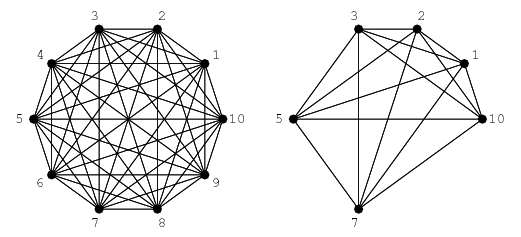
\includegraphics[width=0.6\textwidth]{InducedSubgraph_900.png}
\end{figure}

Spanning subgraphs contain all vertices of the original graph.

\begin{figure}[htb]
    \caption{A graph and a spanning subgraph}
    \centering
    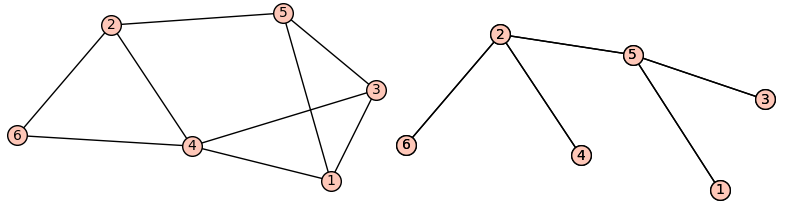
\includegraphics[width=0.6\textwidth]{fig-subgraphs.png}
\end{figure}

Isomorphic graph

\begin{itemize}
    \item A graph $(V', E')$ is isomorphic to $(V, E)$ if there exists a bijection $f: V \rightarrow V'$ such that $(v_i, v_j) \in E$ iff $(f(v_i), f(v_j)) \in E'$
    \item Basically, two isomorphic graphs have the same structure but may have different labels for the vertices
    \item Check if two graphs are isomorphic by mapping corresponding vertices of $V$ to those of $E$
\end{itemize}

Tournament graph: A directed graph that has zero loops and there is only one edge between any two vertices.

Complete/round-robin tournament graph: A tournament graph where all pairs of distinct vertices are connected by one edge.

Single-elimination tournament graph: A tournament graph where: one vertex called the champion has no edge terminating at it, every other vertex is the terminal vertex of exactly one edge, and there is a path from the champion vertex to every other vertex.

\begin{figure}[htb]
    \caption{A single-elimination tournament graph}
    \centering
    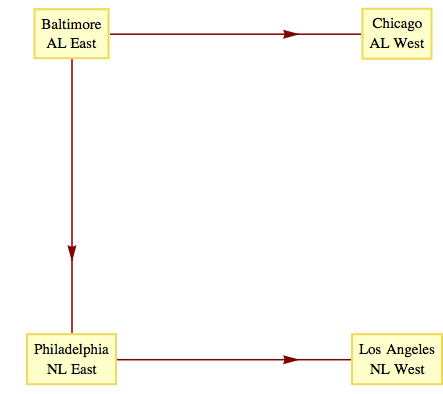
\includegraphics[width=0.4\textwidth]{fig-mlb-1983-9-1.png}
\end{figure}

Bipartite graph: A graph is bipartite if its vertices can be divided into two disjoint and independent sets. Visually, there exists a pair of sets of where a line between the pair cuts all edges.

\begin{figure}[htb]
    \caption{A bipartite graph and its two vertex sets}
    \centering
    \includesvg[width=0.4\textwidth]{Simple-bipartite-graph.svg}
\end{figure}

Degree sequence: A non-increasing sequence of its vertex degrees.

\begin{figure}[htb!]
    \caption{The degree sequence of this graph is $(4, 3, 2, 2, 1)$}
    \centering
    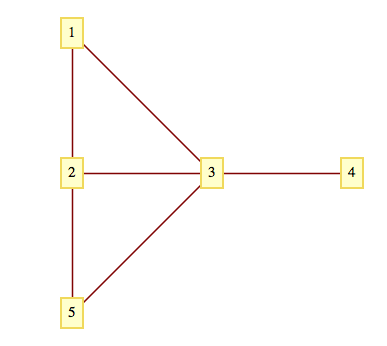
\includegraphics[width=0.5\textwidth]{fig-degrees-example-9-1.png}
\end{figure}

Graphic sequence: A degree sequence is graphic if there exists an undirected graph that has the same degree sequence. As an example, $(3, 3, 1)$ is not a graphic sequence.

The complement of a graph $G = (V, E)$ is $\bar{G} = (V, K - E)$.

Eulerian path
\begin{itemize}
    \item A trail that visits every edge in a graph exactly once
    \item A graph has an Eulerian path iff it has exactly 0 or 2 vertices with odd degrees
    \item Eulerian circuit: A closed Eulerian path
    \item A graph has an Eulerian circuit iff the degrees of all vertices are even
\end{itemize}

Hamilton path
\begin{itemize}
    \item A path that visits each vertex exactly once
    \item Hamilton cycle/Hamiltonian graph: A Hamilton path that is a cycle
\end{itemize}

Distance
\begin{itemize}
    \item Distance: Number of edges in a shortest path connecting a pair of vertices
    \item Eccentricity: Greatest distance between a given vertex and any other vertex
    \item Center: The vertex with the minimum eccentricity
    \item Radius: Minimum eccentricity of any vertex
    \item Diameter: Maximum eccentricity of any vertex
\end{itemize}

\section{Trees}

Tree
\begin{itemize}
    \item An undirected graph that is connected and has no cycles
    \item A disconnected graph that has no cycles is a forest
\end{itemize}

Dijkstra's algorithm: An algorithm for finding the shortest path(s) between all or a pair of vertices in a graph.

Image credits: Al Doerr, Ken Levasseur - Applied Discrete Structures

\end{document}

